\section{ОБЗОР ЛИТЕРАТУРЫ}
\label{sec:domain}

\subsection{Обзор существующих аналогов}
\label{sub:domain:analogs}

\subsubsection{Windows Toop Help}
\label{sub:domain:analogs:windows}

Одним из интерфейсов получения информаци о процессах и потоках в операционной
системе Windows является библиотека Tool Help\cite{tool_help_article}. Ядром
библиотеки является поняние снимка. Снимок является копией только для чтения
одного или нискольких списков, находящихся в системной памяти:
процессы, потоки, модули и кучи.

Процессы, использующие функции Tool Help, получают доступ к этим спискам из
моментальных снимков, а не непосредственно из операционной системы.
Непосредственно сами списки в системной памяти постоянно изменяются, когда
процессы запускаются и завершаются, потоки создаются и уничтожаются, исполняемые
модули загружаются и выгружаются из системной памяти, а кучи создаются и
уничтожаются. Использование информации из снимка предотвращает несоответствия и
гонки. В противном случае изменения в списке могут привести к тому, что поток
будет неправильно перемещаться по списку или вызвать General Protection Fault.
Например, если приложение обходит список потоков, когда другие потоки создаются
или завершаются, информация, которую приложение использует для перемещения по
списку потоков, может устаревать и может вызвать ошибку для приложения,
перемещающегося по списку.

Снимок создаётся функцией \texttt{CreateToolhelp32Snapshot}. Она имеет слудующее
определение\cite{win_tool_help}:

\medskip
\begin{adjustwidth}{\fivecharsapprox}{}
\begin{lstlisting}[basicstyle=\small\ttfamily]
HANDLE WINAPI CreateToolhelp32Snapshot(
  _In_ DWORD dwFlags,
  _In_ DWORD th32ProcessID
);
\end{lstlisting}
\end{adjustwidth}
\medskip

Предоставляется возможным управление содержимым снимка, указав одно или
несколько следующих констант в параметре \texttt{th32ProcessID} при вызове
функции:
\begin{itemize}
\item \texttt{TH32CS\_SNAPHEAPLIST};
\item \texttt{TH32CS\_SNAPMODULE};
\item \texttt{TH32CS\_SNAPPROCESS};
\item \texttt{TH32CS\_SNAPTHREAD}.
\end{itemize}

Флаги \texttt{TH32CS\_SNAPHEAPLIST} и \texttt{TH32CS\_SNAPMODULE} применими при
получении информации об одном процессе. Когда эти значения указаны, списки кучи
и модулей указанного процесса включаются в снимок. При передаче нуля в качестве
идентификатора процесса, используется текущий процесс. При передаче флага
\texttt{TH32CS\_SNAPTHREAD} всегда создается общесистемный снимок, даже если
передан валидный идентификатор процесса.

Для получения состояния куч или модулей всех процессов, передаётся флаг
\texttt{TH32CS\_SNAPALL} и идентификатор текущего процесса. Затем для каждого
дополнительного процесса в снимке снова необходимо вызывать функцию
\texttt{CreateToolhelp32Snapshot} с указанием его идентификатора и флаг
\texttt{TH32CS\_SNAPHEAPLIST} или \texttt{TH32CS\_SNAPMODULE}.

При прохождении по списку процессов используется внутренний итератор. Для
получения информации о первом процессе в списке, используется функция
\texttt{Process32First}. Для дальнейшего перемещения по списку процессов для
последующих записей используется функция \texttt{Process32Next}. Обе функции
заполняют структуру \texttt{PROCESSENTRY32} информацией о процессе в из снимка.
Структура \texttt{PROCESSENTRY32} имеет следующее определение:

\medskip
\begin{adjustwidth}{\fivecharsapprox}{}
\begin{lstlisting}[basicstyle=\small\ttfamily]
typedef struct tagPROCESSENTRY32 {
  DWORD     dwSize;
  DWORD     cntUsage;
  DWORD     th32ProcessID;
  ULONG_PTR th32DefaultHeapID;
  DWORD     th32ModuleID;
  DWORD     cntThreads;
  DWORD     th32ParentProcessID;
  LONG      pcPriClassBase;
  DWORD     dwFlags;
  TCHAR     szExeFile[MAX_PATH];
} PROCESSENTRY32, *PPROCESSENTRY32;
\end{lstlisting}
\end{adjustwidth}
\medskip

Как видно из определения, предоставленный разработчиками системы интерфейс
позволяет получить такие параметры процесса, как идентификатор, число потоков,
идентификатор родительского процесса, базовый приоритет созданных данным
просцессом потоков, имя исполняемого файла процесса. Четыре поля структуры
больше не используются, что показывает важность и серьёзность построения
интерфейса, по возможности устойчивого к изменениям архитектуры системы, при
которых элементы существующего интерфейса теряют смысл.

\subsubsection{Apple macOS}
\label{sub:domain:analogs:macos}

Несмотря на то, что система macOS является прямым потомком UNIX, она не имеет
собственной реализации \texttt{procfs}. Такие утилиты как \texttt{ps} используют
вместо этого интерфейсы kvm и sysctl\cite{osxproc}. Кроме того, предоставляется
системная библиотека libproc.h, а ныне устаревшие версии macOS для сбора
информации о процессах имели интерфейс Process Manager.

Process Manager ведет список всех открытых процессов\cite{procmanag}. Получение
элементов списка производится вызовами функции \texttt{GetNextProcess}. Такой
интерфейс похож на решение в ОС Microsoft Windows, однако не требует создания
снимка, а в качестве единственного аргумента принимает последний валидный
идентификатор процесса, возвращенный одной из функций % \texttt{GetNextProcess},
\texttt{LaunchApplication}, \texttt{GetFrontProcess}, \texttt{GetCurrentProcess}
или константу \texttt{kNoProcess} в начале хождения по списку. Порядок, в
котором будут предоставляться идентификаторы, жёстко не регламентирован и
является внутренним для Process Manager. Кроме того, полученный идентификатор
процесса можно использовать только в других функциях Process Manager.

Для получения информации о конкретном процессе в Process Manager используется
функция \texttt{GetProcessInformation}. Кроме полученного ранее инденитфикатора
процесса в функцию передаётся указатель на структуру \texttt{ProcessInfoRec}, в
которую будет помещена информация о процессе. Структура имеет следующее
определение:

\medskip
\begin{adjustwidth}{\fivecharsapprox}{}
\begin{lstlisting}[basicstyle=\small\ttfamily]
TYPE ProcessInfoRec =
   RECORD
      processInfoLength:   LongInt;
      processName:         StringPtr;
      processNumber:       ProcessSerialNumber;
      processType:         LongInt;
      processSignature:    OSType;
      processMode:         LongInt;
      processLocation:     Ptr;
      processSize:         LongInt;
      processFreeMem:      LongInt;
      processLauncher:     ProcessSerialNumber;
      processLaunchDate:   LongInt;
      processActiveTime:   LongInt;
      processAppSpec:      FSSpecPtr;
   END;
\end{lstlisting}
\end{adjustwidth}
\medskip

В структуре водержится, имя и идентификатор процесса, тип и подпись процесса,
адрес раздела с процессом, размер свободной памяти в куче, идентификатор
родительского процесса, время запуска процесса, накопленное процессорное время и
расположение исполняемого файла процесса. Кроме этого, имеются флаги, которые
описывают, является ли процесс приложением или Desk Accessory.

Библиотека libproc.h предоставляет бинарный интерфейс, дающий возможность
различную информацию, не привязываясь к внутренним структурам данных, так как
используются либо типы, определённые в стандарте POSIX, либо структуры,
определённые специально только для передачи информации пространству
пользователя\cite{libproc}. Определения некоторых функций:

\medskip
\begin{adjustwidth}{\fivecharsapprox}{}
\begin{lstlisting}[basicstyle=\small\ttfamily]
int	proc_listpidspath(uint32_t	type,
			  uint32_t	typeinfo,
			  const char	*path,
			  uint32_t	pathflags,
			  void		*buffer,
			  int		buffersize);
int proc_listpids(uint32_t type, uint32_t typeinfo,
                  void *buffer, int buffersize);
int proc_listallpids(void * buffer, int buffersize);
int proc_listpgrppids(pid_t pgrpid,
                      void * buffer, int buffersize);
int proc_listchildpids(pid_t ppid,
                       void * buffer, int buffersize);
int proc_pidinfo(int pid, int flavor, uint64_t arg,
                 void *buffer, int buffersize);
int proc_pidfdinfo(int pid, int fd, int flavor,
                   void * buffer, int buffersize);
int proc_pidfileportinfo(int pid, uint32_t fileport,
        int flavor, void *buffer, int buffersize);
\end{lstlisting}
\end{adjustwidth}
\medskip

Такой подход является более устойчивым к изменениям внутренней архитектуры ядра,
при нём маловероятна ситуация, когда большая часть полей структуры больше нет
смысла использовать, как это произошло с Tool Help в Windows. Кроме того, такие
функции достаточно расширяемы засчёт параметра, определяющего тип результирующих
данных, необходимых пользовательской программе.

\subsection{Аналитический обзор}
\label{sub:domain:analitic_overview}

Очень критическая ситуация произошла с мужчиной на рисунке \ref{fig:perf_bug}.

\begin{figure}
  \centering
  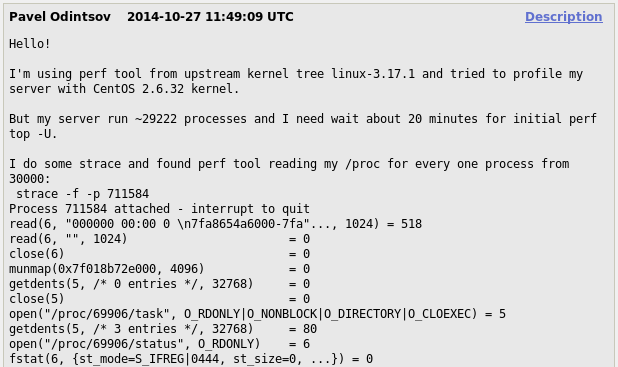
\includegraphics[scale=0.7]{perf_bug.png}
  \caption{Сообщение о низкой производительности в багтрекере ядра\cite{slowperf}}
  \label{fig:perf_bug}
\end{figure}

\nocite{
  kernel_docs,
  rlove,
  understanding,
  tanenbaum,
  johnson,
  kernelnewbies,
  vagin,
  lkml,
  anatomy,
  lwn,
  map,
  greg,
  profarch,
  man_syscall}
